Cílem práce bylo navrhnout a implementovat webovou aplikaci umožňující stažení 3D modelů dílů LEGO. Tento cíl byl úspěšně naplněn včetně zveřejnění aplikace do sítě internet. 

Instance aplikace je nasazena a připravena k~používání na adrese \url{http://printabrick.org}. 


\begin{figure}[htbp]
    \centering
    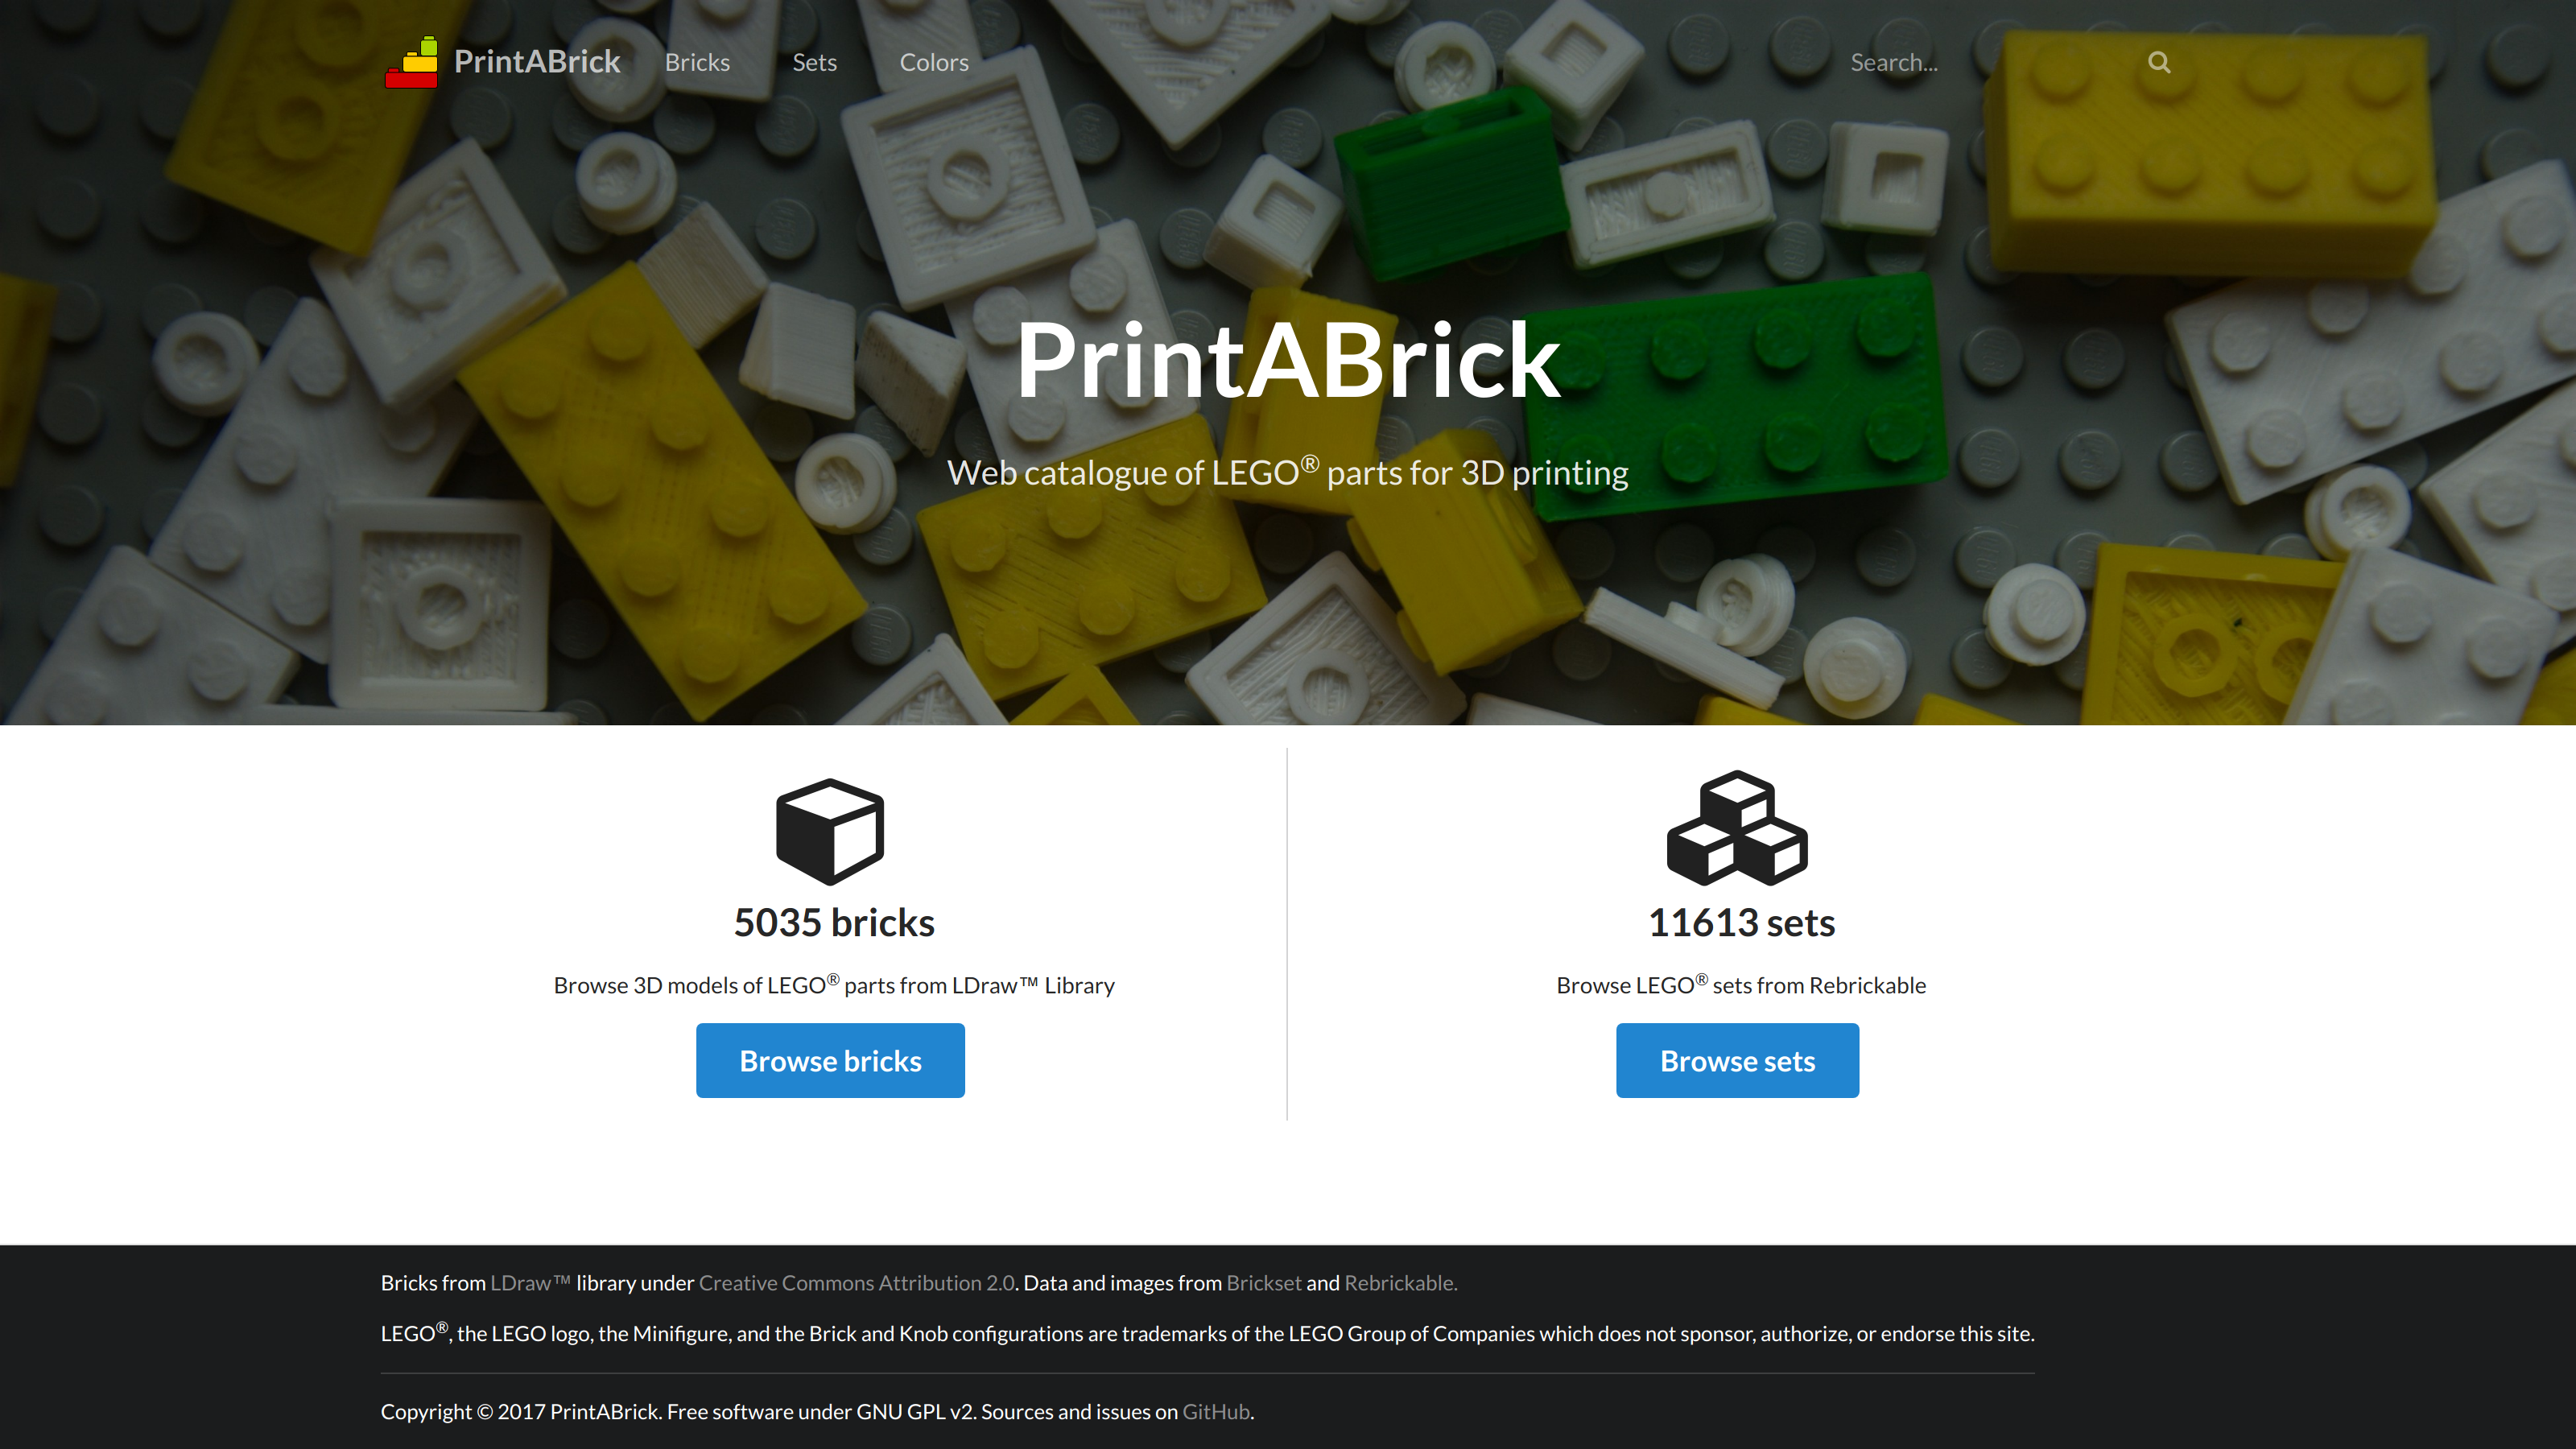
\includegraphics[width=\textwidth,height=\textheight,keepaspectratio]{images/screenshot-homepage.png}
    \caption{Snímek obrazovky – domovská stránka\label{facebook-share}}
\end{figure}

\begin{figure}[htbp]
    \centering
    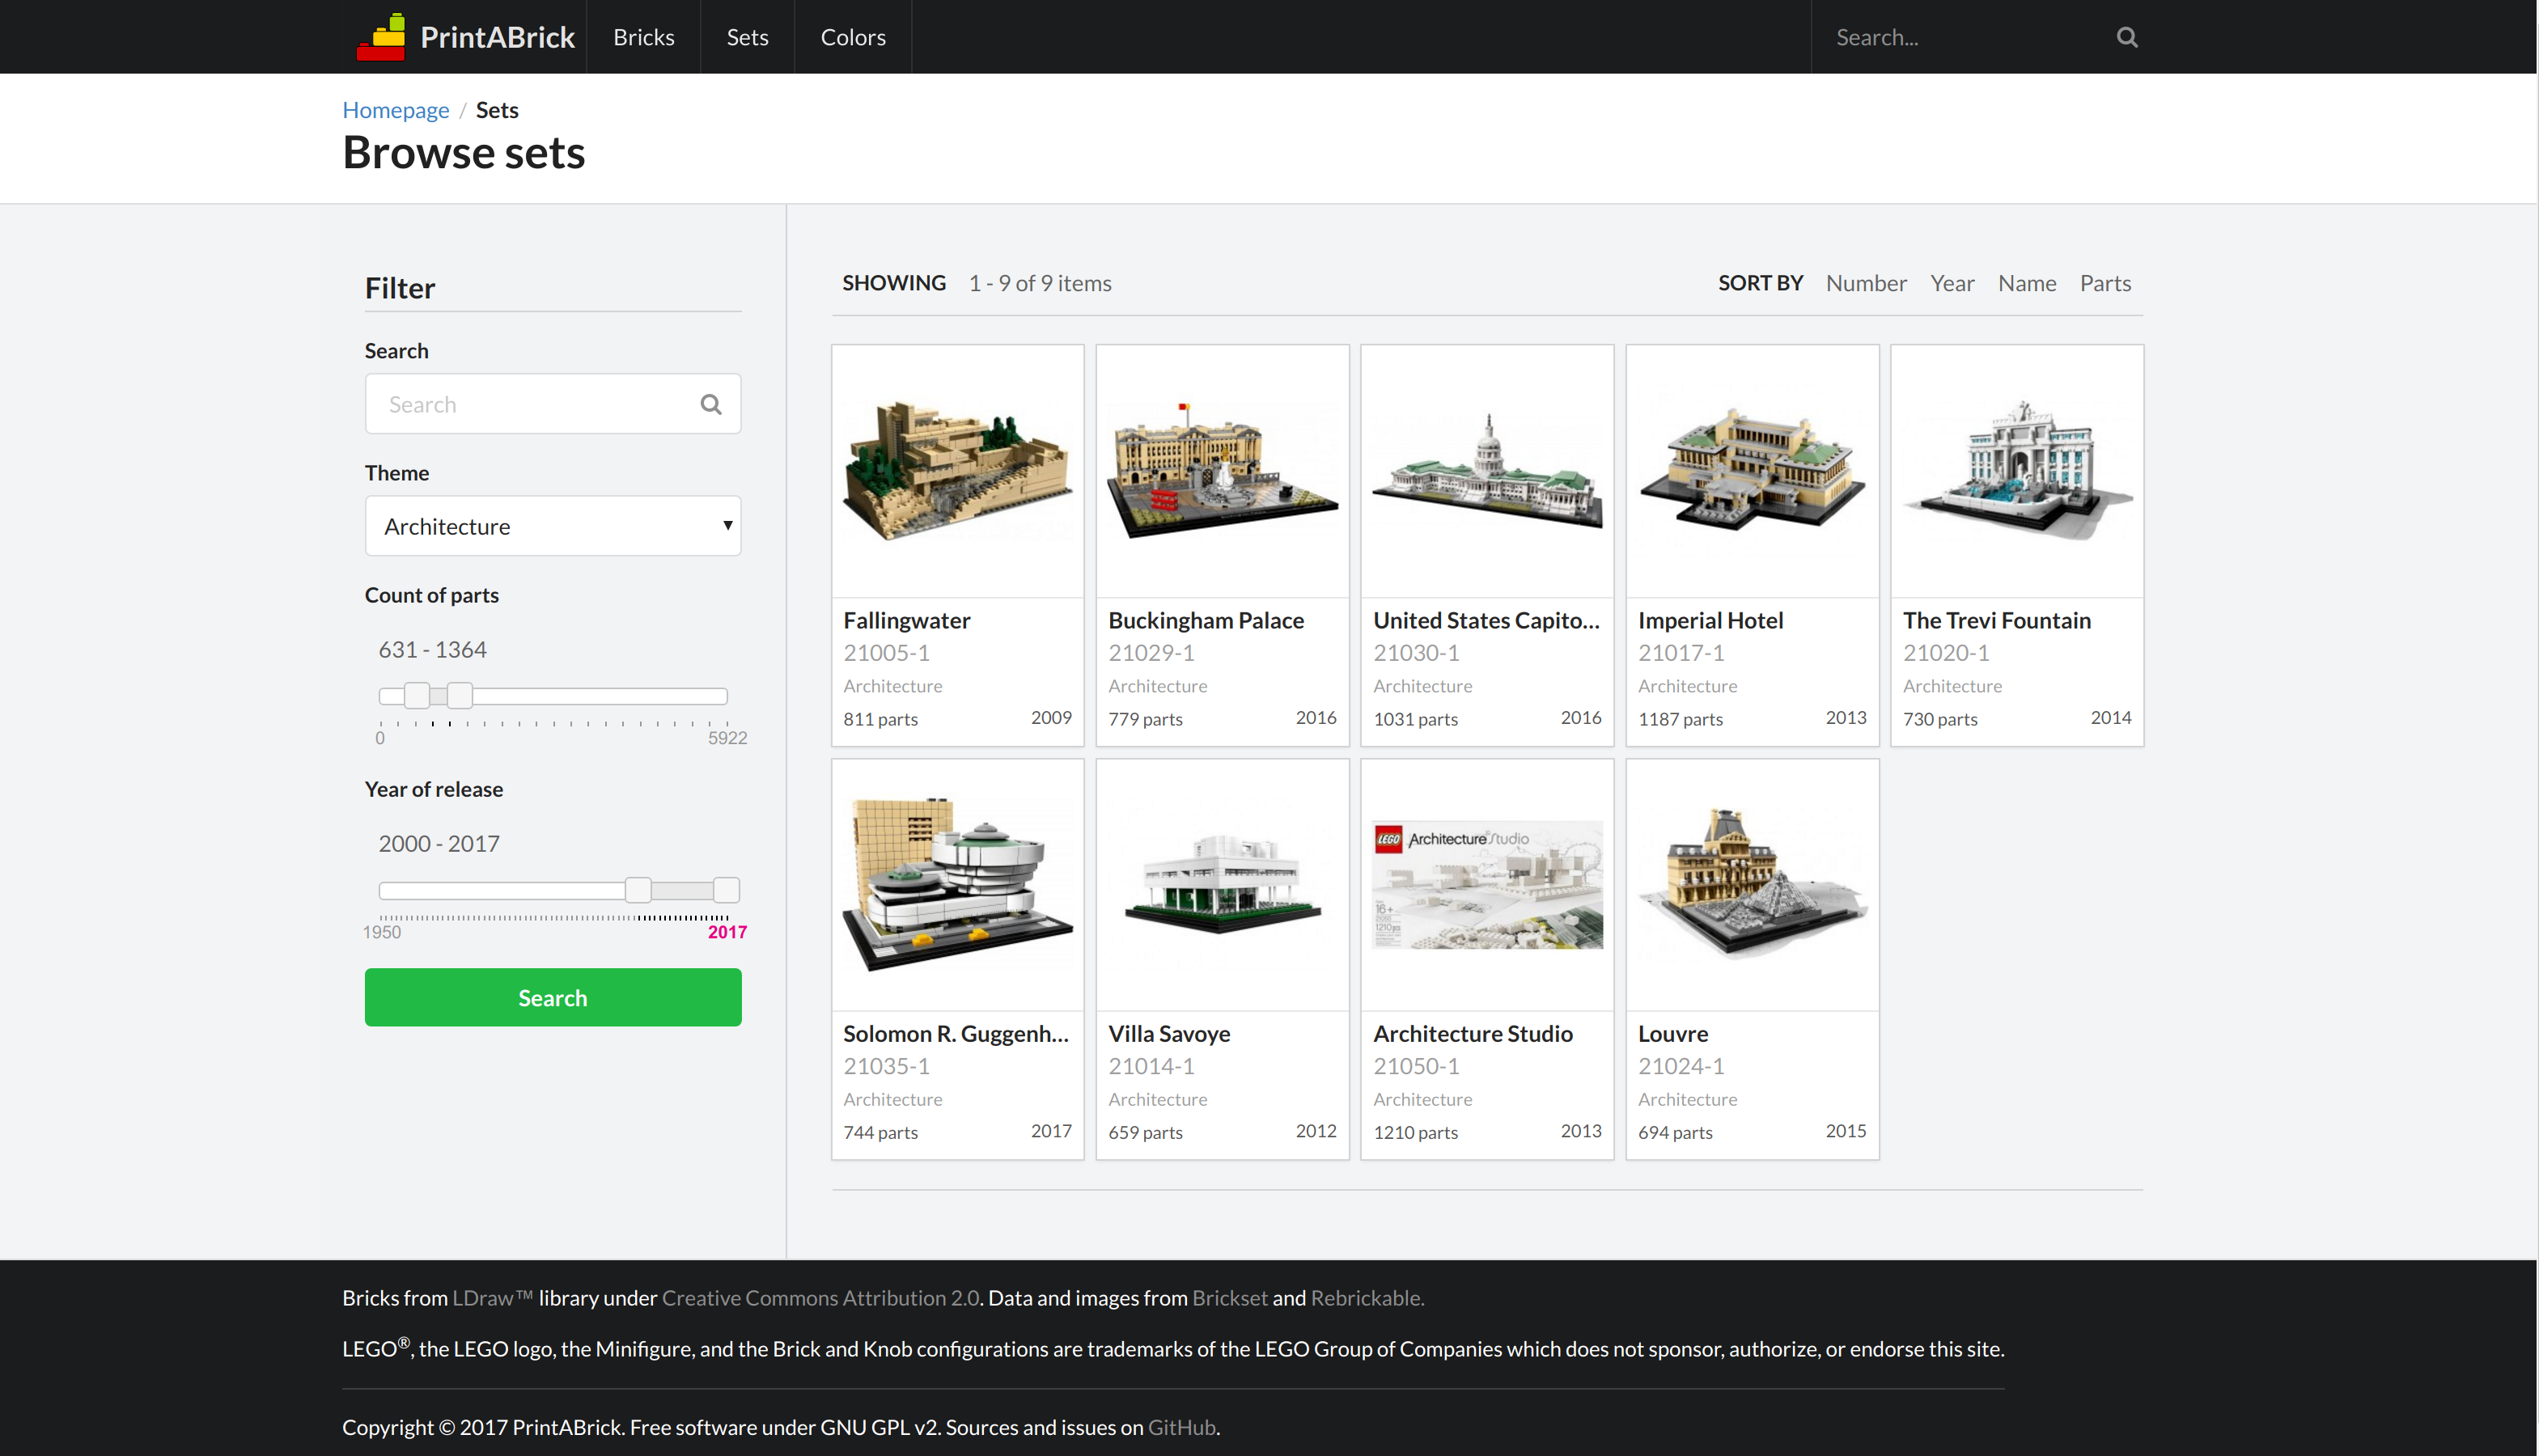
\includegraphics[width=\textwidth,height=\textheight,keepaspectratio]{images/screenshot-sets.png}
    \caption{Snímek obrazovky – výpis stavebnic\label{facebook-share}}
\end{figure}

\subsubsection*{Možnosti dalšího rozvoje}\label{moznosti-dalsiho-rozvoje}

V~rámci možností dalšího rozvoje aplikace vidím následující:
\begin{itemize}
    \item výpočet odhadu množství materiálu potřebného k~tisku,
    \item implementace správy sbírek 
\end{itemize} 
